В модуле со средствами для разработки задач, как и во всех остальных модулях, классы распределены по пакетам. Отдельные пакеты отведены под классы для работы с генераторами, валидаторами и чекерами, а также "--- под вспомогательные классы и для одного класса логгирования. На рис.~\ref{package_diagram_development} изображена схема расположения классов в данном модуле.

\begin{figure}[h]
\center{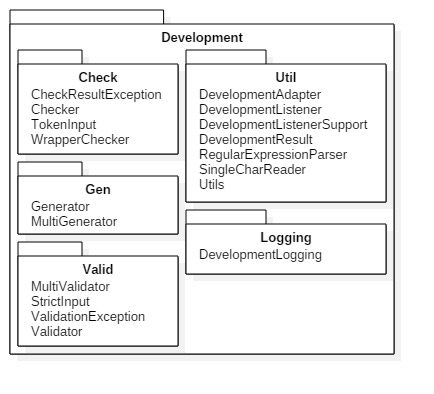
\includegraphics[scale=0.8]{package_diagram_development}}
\caption{Модуль для разработки задач}
\label{package_diagram_development}
\end{figure}

Начнём с рассмотрения классов, предназначенных для автоматической генерации тестов. Абстрактный класс \texttt{Generator} "--- один из тех классов, которые пользователь должен будет расширить, написав дополнительный код. В данном классе нужно реализовать всего один защищённый метод \texttt{generate(String[]~args)}, принимающий произвольное количество строковых аргументов, которые можно использовать внутри помещаемой в метод логики генерации отдельного теста. Также в классе \texttt{Generator} доступно множество реализованных защищённых методов, которые можно вызывать из пользовательского кода. Например, есть методы для вывода чисел и строк в выходной поток и методы для получения псевдослучайных чисел или символов. Методом \texttt{getOutput()} можно получить объект класса \texttt{PrintStream} из стандартной библиотеки и делать весь вывод в него, поскольку он весьма удобен.

Внутри объекта класса \texttt{Generator} хранится один объект класса \texttt{Random} для генерации псевдослучайных чисел, который инициализируется один раз в момент создания генератора (при этом есть возможность самому выбрать значение \texttt{random\-Seed}), и в дальнейшем для получения любых случайных значений используется он один. Более того, он сохраняется между отдельными вызовами метода \texttt{generate()}, что обеспечивает однозначность вывода сгенерированных подряд тестов.

Среди реализованных методов класса \texttt{Generator} есть удобные методы вроде \texttt{nextInt(int~lowerBound, int~higherBound)} для большинства простых типов Java, позволяющие получить случайное число из заданного диапазона. Также присутствуют методы наподобие \texttt{any(int[]~values)}, возвращающие некоторое число из передаваемого массива значений, и, к примеру, метод \texttt{anyLine(String regular\-Expression, int~length)} для получения случайной строки из символов, удовлетворяющих регулярному выражению (о таких выражениях подробнее речь пойдёт ниже).

Класс \texttt{MultiGenerator} предназначен для многократного запуска одного и того же генератора. Объект данного класса получает массив путей к файлам для генерации, аргументы, которые нужно передать генератору, а также инициализирующее значение для объекта класса \texttt{Random}. Каждый вызов метода \texttt{generate()} происходит в отдельном потоке, чтобы в случае слишком долгого выполнения его можно было остановить.

Теперь рассмотрим классы для валидации тестов. Поскольку для валидатора важно строго относиться к пробелам и переносам строки во входном файле, для их удобной обработки были написаны специальные классы \texttt{Single\-Char\-Reader} и \texttt{Strict\-Input}. Первый из них необходим для преодоления ограничений стандартного класса \texttt{Buffered\-Reader}, который, к примеру, не позволяет посмотреть следующий элемент из входного потока, оставляя курсор на прежнем месте. Класс \texttt{Strict\-Input} предоставляет множество методов вроде \texttt{readInt()}, \texttt{readSpace()}, \texttt{readln()}, \texttt{readEof()}, считывающих отдельные элементы входного файла. Методом \texttt{getState()} можно получить объект, содержащий краткую информацию о положении курсора во входном файле: номер строки и количество считанных в ней символов.

Абстрактный класс \texttt{Validator} содержит метод \texttt{validate(String[]~args)}, который необходимо реализовать пользователю. Валидатор, как и генератор, может принимать строковые аргументы, но также он может выбрасывать исключение типа \texttt{Validation\-Exception}, в которое можно записать текущее положение курсора и некоторое сообщение об ошибке. Методом \texttt{getInput()} получается объект класса \texttt{Strict\-Input} для строгого считывания ввода. Также доступны методы, упрощающие валидацию, такие, как \texttt{inBounds(int~lowEdge, int~number, int~highEdge} для проверки, что число принадлежит диапазону, или \texttt{matches\-Expression(String~line, String~regular\-Expression)} для проверки, что все символы строки удовлетворяют регулярном выражению.

По аналогии с генераторами присутствует класс \texttt{Multi\-Validator} для валидации нескольких тестов подряд в помощью одного и того же валидатора, а также "--- для проведения валидации в отдельном потоке.

Перейдём к рассмотрению классов для проверки корректности полученного ответа. Поскольку в чекере не нужно строго проверять формат считываемых данных, в них используется другой класс для ввода значений "--- \texttt{Token\-Input}, "--- который считывает значения по одной лексеме за раз, пропуская пробелы и переносы строк.

Абстрактный класс \texttt{Checker} содержит метод \texttt{check()}, подлежащий реализации в расширяющем классе. Этот метод всегда должен информировать вызывающий код о результате проверки посредством выброса исключения типа \texttt{Check\-Result\-Exception}. Такое решение было принято для того, чтобы вернуть результат можно было не только из самого метода \texttt{check()}, но и из любого другого метода вниз по стеку вызовов. В исключении \texttt{Check\-Result\-Exception} можно сохранить вердикт проверки (одна из констант \texttt{OK}, \texttt{WRONG\_ANSWER} и \texttt{FAIL}) и сообщение.

В методе \texttt{check()} тремя методами \texttt{getInput()}, \texttt{getOutput()} и \texttt{getAnswer()} можно получить объекты класса \texttt{Token\-Input}, соответственно, для файлов с входными данными, с ответом участника и с ответом жюри. Также есть методы для завершения проверки с некоторым вердиктом при выполнении или невыполнении заданного условия.

Присутствует класс \texttt{Wrapper\-Checker}, представляющий собой обёртку над объектом класса, расширяющего \texttt{Checker}, необходимую для автоматического выполнения кода чекера в отдельном потоке.

В каждом из классов \texttt{Generator}, \texttt{Validator} и \texttt{Checker} находится метод \texttt{getParser()}, который возвращает объект класса \texttt{RegularExpressionParser}. Этот класс предоставляет методы для определения, удовлетворяют ли все символы строки некоторому выражению, и для получения символа, удовлетворяющего выражению. Запросы кэшируются, поэтому можно делать много запросов с одним выражением, и они будут быстро обрабатываться.

Поддерживается простой синтаксис выражений, позволяющий одной строкой задать группу разрешённых символов. С помощью фигурных скобок можно указать группу подряд идущих в алфавите символов, а с помощью знака <<\%>> можно экранировать символы скобок. Например, чтобы выбрать все латинские символы, все цифры, круглые и фигурные скобки, достаточно сделать строку:

\begin{center}
\texttt{[a-z][A-Z][0-9]()\%[\%]}
\end{center}

Также в каждом из классов \texttt{Multi\-Generator}, \texttt{Multi\-Validator} и \texttt{Wrapper\-Checker} встроена система слушателей. Объект класса \texttt{Development\-Listener\-Sup\-port} содержит набор слушателей \texttt{Development\-Listener}, уведомляемых о начале и об окончании некоторого процесса (например, генерации или валидации тестов), а также о начале и об окончании обработки каждого отдельного теста. Эта система используется в модуле взаимодействия с пользователем для вывода сообщений на экран параллельно с процессом обработки тестов.

Наконец, класс \texttt{Utils} содержит обобщённый метод \texttt{getSupplier()}, реализующий рутинный код для загрузки класса в виртуальную машину Java во время выполнения.